%!TEX TX-program = xelatex
\documentclass[8pt]{article}
\usepackage{allan-eason}

\usetikzlibrary{positioning}
\usetikzlibrary{svg.path}

\graphicspath{ {./images/} }

\author{\normalfont\sffamily\large\bfseries{高一(4)班\ 邵亦成\ 48号}}
\title{\normalfont\sffamily\huge\bfseries{\textcolor{allanblue}{220330}\ \textcolor{allancyan}{三角函数}\ 题目选解}}
\date{}

\geometry{a4paper, scale=0.8}

\lhead{\textcolor{allanblue}{220330}\ \textcolor{allancyan}{三角函数}\ 题目选解}

\begin{document}

	\maketitle

	\section{填空题}
		\defword{1. }$\displaystyle \max_{x\in\RR}{\left(2\sin x-1\right)}=\ansmath{1}$, 此时$x\in\ansmath{\left\{x|x=2k\pi+\dfrac{\pi}{2}, k\in\ZZ\right\}}$.

		\answord{解析. }三角函数的极值性.
		~\\

		\defword{2. }$\displaystyle \min_{x\in\RR}{\left(-3\cos x+5\right)}=\ansmath{2}$, 此时$x\in\ansmath{\left\{x|x=2k\pi, k\in\ZZ\right\}}$.

		\answord{解析. }三角函数的极值性.
		~\\

		\defword{3. }函数$\displaystyle y=3\cos\left(\frac{1}{2}x+\frac{\pi}{4}\right)$的周期是$T=\ansmath{4k\pi, k\in\ZZ, k\neq 0}$.

		\answord{解析. }三角函数的周期性.
		~\\

		\defword{4. }在$\triangle ABC$中, $a=12, A=45\degree, C=60\degree$, 则$b=\ansmath{6+6\sqrt{3}}$.

		\answord{解析. }解三角形.
		~\\

		\defword{5. }在$\triangle ABC$中, $a=4, b=5, S_{\triangle}=5\sqrt{3}$, 则$c=\ansmath{\sqrt{21} \lgor \sqrt{61}}$.

		\answord{解析. }解三角形.
		~\\

		\defword{6. }函数$y=3\sin\left(2x+\dfrac{\pi}{3}\right)$的单调递增区间是$\displaystyle\ansmath{\bigcup_{k\in\ZZ}{\left[k\pi-\frac{5\pi}{12}, k\pi+\frac{\pi}{12}\right]}}$.

		\answord{解析. }三角函数的单调性.
		~\\

		\defword{7. }函数$y=5\sin x+\cos 2x$的值域是$\ansmath{[-6, 4]}$.

		\answord{解析. }三角变换, 二次函数.
		~\\

		\defword{8. }函数$y=\sin x +\sqrt{3} \cos x, x\in\left[-\dfrac{\pi}{6}, \dfrac{\pi}{3}\right]$的值域是$\ansmath{[1, 2]}$.

		\answord{解析. }三角函数的值域; 三角变换.
		~\\

		\defword{9. }在$\triangle ABC$中, $AB=\sqrt{3}, BC=3, AC=4$, 则$AC$边上的中线$BD=\ansmath{\sqrt{2}}$.

		\answord{解析. }解三角形.
		~\\

		\defword{10. }在$\triangle ABC$中, 若$\sin A:\sin B:\sin C=3:5:7$, $S_{\triangle ABC}=15\sqrt{3}$, 则最长的边长为$\ansmath{14}$.

		\answord{解析. }解三角形; \athword{海伦$\cdot$秦九韶公式}.
		~\\

		\defword{11. }设函数$f(x)$是以$2$为周期的奇函数, 且$f\left(-\dfrac{2}{5}\right)=7$. 若$\sin \alpha = \dfrac{\sqrt{5}}{5}$, 则$f(4\cos 2\alpha)=\ansmath{-7}$.

		\answord{解析. }三角变换, 函数的基本性质.
		~\\

		\defword{12. }已知函数$f(x)=\dfrac{1}{2}\left(\sin x+\cos x\right)-\dfrac{1}{2}\abs{\sin x-\cos x}$, 则$f(x)$的值域是$\ansmath{\left[-1, \dfrac{\sqrt{2}}{2}\right]}$.

		\answord{解析. }三角函数的值域; 分段函数.

	\section{解答题}
		\defword{13. }在$\triangle ABC$中, $a, b, c$分别是三个内角$A, B, C$的对边. 若$a=2, C=\dfrac{\pi}{4}, \cos\dfrac{B}{2}=\dfrac{2\sqrt{5}}{5}$, 求$S_{\triangle ABC}$.

		\answord{解析. }解三角形. 过程略. $S_{\triangle ABC}=\ansmath{\dfrac{8}{7}}$.
		~\\

		\defword{14. }在$\triangle ABC$中, 内角$A, B, C$所对的边长分别是$a, b, c$.

		\begin{enumerate}[label=(\arabic*)]
			\item 若$c=2, C=\dfrac{\pi}{3}, S_{\triangle ABC}=\sqrt{3},$求$a, b$.
				~\\

				\answord{解析. }解三角形. 过程略. $\ansmath{a=b=2}$.

			\item 若$\sin C + \sin (B-A) = \sin 2A$, 试判断$\triangle ABC$的形状.
				~\\

				\answord{解析. }解三角形, 三角变换.

				\begin{align*}
					A+B+C=\pi &\Rightarrow \sin C=\sin (A+B)\\
					&\Rightarrow \sin(A+B)+\sin(B-A) = 2\sin A \cos A\\
					&\Rightarrow 2\sin B\cos A = 2\sin A\cos A\\
					&\Rightarrow \cos A=0 \lgor \sin B = \sin A\\
					&\Rightarrow A=\frac{\pi}{2} \lgor A=B\\
					&\Rightarrow \triangle ABC \text{是} \ansmath{\Rt \triangle \lgor \text{等腰} \triangle}.
				\end{align*}	
		\end{enumerate}
		~\\

		\defword{15. }已知函数$f(x)=2-\sin \left(2x+\dfrac{\pi}{6}\right)-2\sin^2 x, x\in \RR$,

		\begin{enumerate}[label=(\arabic*)]
			\item 求函数$f(x)$的最小正周期.
				~\\

				\answord{解析. }三角函数的周期性; 三角变换. 过程略. $\displaystyle \min_{T>0}T=\ansmath{\pi}$.

			\item 求$f(x)$单调递增区间.
				~\\

				\answord{解析. }三角函数的单调性. 过程略. $\displaystyle\ansmath{\bigcup_{k\in\ZZ}\left[k\pi - \frac{2}{3}\pi, k\pi - \frac{\pi}{6}\right]}$.

			\item 记$\triangle ABC$的内角$A, B, C$的对边长分别为$a, b, c$, 若$f\left(\dfrac{B}{2}\right)=1, b=1, c=\sqrt{3}$, 求$a$的值.
				~\\

				\answord{解析. }解三角形, 三角方程.

				由$f\left(\dfrac{B}{2}\right)=1$可知$B=\dfrac{\pi}{6}$.

				考虑到$b=1, c=\sqrt{3}$, 又由正弦定理有$\dfrac{b}{\sin B}=\dfrac{c}{\sin C}$, 可知$\sin C=\dfrac{\sqrt{3}}{2}$, 故可知$C=\dfrac{\pi}{3} \lgor \dfrac{2\pi}{3}$.

				当$C=\dfrac{\pi}{3}, A=\dfrac{\pi}{2}, a=\sqrt{b^2+c^2}=2$.

				当$C=\dfrac{2\pi}{3}, A=\dfrac{\pi}{6}, B=\dfrac{\pi}{6}, a=b=1$.

				于是有$\ansmath{a=1 \lgor 2}$.
		\end{enumerate}

	\section{附加题}
		\defword{16. }如图所示, $ABCD$是一块边长为$7$米的正方形铁皮, 其中$ATN$是一半径为$6$米的扇形, 已经被腐蚀不能使用, 其余部分完好可利用. 工人师傅想在未被腐蚀部分截下一个有边落在$BC$与$CD$上的长方形铁皮$PQCR$, 其中$P$是$\arc{TN}$上一点. 设$\angle TAP = \theta$, 长方形$PQCR$的面积为$S$平方米.
		
		$$
		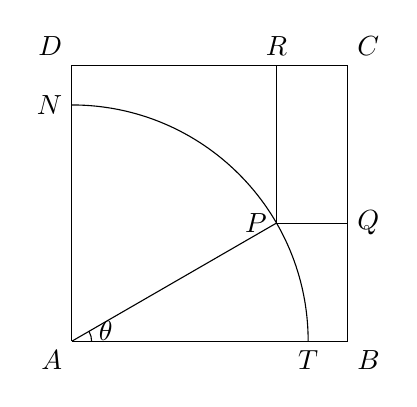
\begin{tikzpicture}[scale=0.5, baseline=0]
    		\draw[black] (0, 0)--(7, 0)--(7, 7)--(0, 7)--(0, 0) node at (0, 0) [anchor=north east] {$A$} node at (7, 0) [anchor=north west] {$B$} node at (7, 7) [anchor=south west] {$C$} node at (0, 7) [anchor=south east] {$D$};
    		\draw[black] (6, 0) arc[start angle=0, end angle=90, radius=6] node at (6, 0) [anchor=north] {$T$} node at (0, 6) [anchor=east] {$N$};
    		\draw[black] (0.5, 0) arc[start angle=0, end angle=30, radius=0.5] node [right] {$\theta$};
    		\draw[black] (0, 0)--({3*sqrt(3)}, 3) node at ({3*sqrt(3)}, 3) [anchor=east]{$P$};
    		\draw[black] ({3*sqrt(3)}, 7)--({3*sqrt(3)}, 3)--(7, 3) node at ({3*sqrt(3)}, 7) [anchor=south] {$R$} node at (7, 3) [anchor=west] {$Q$};
    	\end{tikzpicture}
    	$$

		\begin{enumerate}[label=(\arabic*)]
			\item 求$S$关于$\theta$的函数解析式.

				\answord{解析. }三角比. 过程略. $\ansmath{S=49-42\left(\sin \theta + \cos \theta\right)+36\sin\theta\cos\theta, \theta\in\left[0, \dfrac{\pi}{2}\right]}$.

			\item 求$S$的最大值及此时$\theta$的值.

				\answord{解析. }三角变换; 二次函数.

				令$t=\sin \theta + \cos \theta = \sqrt{2} \sin \left(\theta + \dfrac{\pi}{4}\right), \sin \theta \cos \theta = \dfrac{t^2 - 1}{2}$, 于是有$S=49-42t+18\left(t^2-1\right)=18t^2-42t+31$.

				注意到$\theta \in \left[0, \dfrac{\pi}{2}\right]$, 可知$\theta + \dfrac{\pi}{4} \in \left[\dfrac{\pi}{4}, \dfrac{3\pi}{4}\right]$, 有$t=\sqrt{2}\sin\left(\theta + \dfrac{\pi}{4}\right)\in\left[1, \sqrt{2}\right]$.

				于是有$S=S(t)=18t^2-42t+31=18\left(t-\dfrac{7}{6}\right)^2+\dfrac{13}{2}, t\in\left[1, \sqrt{2}\right],$

				故\answord{$\displaystyle \max_{t\in\left[1, \sqrt{2}\right]}S=\at{S}{t=\sqrt{2}}=67-42\sqrt{2}, $此时$\theta = \dfrac{\pi}{4}$}.

		\end{enumerate}

\end{document}